\documentclass{psu-report}
\usepackage{psu-thesis-chicago}
\usepackage{todonotes}
\usepackage{amsmath,amssymb,amsfonts,amsthm,mathtools}
\usepackage{siunitx}
\usepackage{tikz,pgfplots,pgfplotstable}
\usetikzlibrary{positioning, shapes.geometric}
\pgfplotsset{compat=newest}

\addbibresource{refs.bib}

\title{Organ Pipe Voicing}
\author{
    Meghana Cyanam \\
    Hai Nguyen \\
    Gabriel Pinochet-Soto \\
}
\doctype{report}
\psumonth{April}
\psuyear{2025}

\professorOne{Daniel Taylor-Rodriguez}
\professorTwo{Jacob Schultz}
\clientOne{Arno Patin}

\documentformat{monograph}


\begin{document}

\maketitle
\makecopyright

\begin{psuabstract}
    Intonation, or voicing, in pipe organ technology involves adjusting each
    pipe to produce its optimal sound.
    This process entails determining the appropriate tone that harmonizes with
    the organ’s style, the architectural setting, and the preferences of its
    owner.
    While the “perfect” tone is largely subjective, certain aspects, such as 
    volume and harmony, can be quantified using contemporary tools.
    
    The relationship between the diameter of the pipe’s toe, the size of the toe
    hole, airflow, and frequency is paramount in comprehending and optimizing
    organ pipe performance.
    These parameters interact to influence the pipe’s tonal characteristics,
    acoustic intensity, and harmonic structure. Adjustments in the toe hole size
    regulate airflow, affecting both frequency and tonal balance, while the pipe
    toe diameter significantly shapes the overall sound profile.
    Exploring these connections elucidates the intricacies of voicing and 
    scaling processes, providing insights into both traditional methods and
    contemporary approaches employing acoustic measurements.

    Our goal is to clarify the relationship between the Ising number and the
    parameters of the organ pipe, and to provide a model that can be used to
    dimension the pipes before the voicing stage.
\end{psuabstract}

% \begin{psudedication}
% \end{psudedication}

% \begin{psuacknowledgments}
% \end{psuacknowledgments}

\tableofcontents
\clearpage

\listoftables
\clearpage

\listoffigures
\clearpage

% \begin{psuglossary}
% \begin{description}
%     \item[LaTeX] A document preparation system
% \end{description}
% \end{psuglossary}

% \begin{psupreface}
% \end{psupreface}

\startbody

\chapter{Introduction}

Pipe organs have been around for hundreds of years, and making them sound just
right is a special job called intonation, or \emph{voicing}.
This means adjusting each pipe to create the best sound for the organ.
The way a pipe looks and is built -- like its size, shape, and material-- can
change how it sounds.
These details are decided first, and then the pipes are fine-tuned before being
added to the organ.

Experts have been studying these details for a long time, and they’ve written
about different ways to make pipes sound beautiful and harmonious.
Our goal is to understand how the Ising number -- a special number that helps
with harmonization -- relates to the pipe’s design, how it behaves upon modification of
the airflow, and how we can use this information to:
\begin{enumerate}
    \item Make the Ising number more accurate.
    \item include the flow rate in the Ising number.
    \item Create a model that helps us design pipes before we start intonating them.
\end{enumerate}

\chapter{Action Plan}

In this Chapter, we discuss different approaches for successfully improving the
organ pipe voicing process.
We discuss the project goals and objectives, potential solutions, and the
expected outcomes of the project.
Subsequently, we present the data available, some challenges and concerns that
we encountered.
Proposed methodologies are discussed and briefly explained.
Finally, we present the project timeline and the expected deliverables.

\section{Project Goals and Objectives}

The main goal of this project concerns the improvement of the organ pipe voicing
process.
As the organ pipe design is a complex process, and usually is not a reversible
process, it is important to ensure that the design of the pipes is done
correctly; this presents a key constraint for the intonation process.
The parameters involved are various, which makes learning about this complex
system a difficult task; the understanding of these parameters and their
interactions would facilitate the harmonization process.

A particular subgoal of this project is to improve the Ising
formula~\autocite{1971Ising-1}, which reads
\begin{equation}
    \label{eq:ising}
    \mathsf{I}
    =
    \frac{v}{\omega}\sqrt{\frac{d}{h^3}}
    =
    \frac{1}{\omega}\sqrt{\frac{2 P d}{\rho h^3}},
\end{equation}
where \(\mathsf{I}\) is the Ising number, \(\omega\) is the (target) frequency
of the pipe, \(v\) is the jet initial velocity, \(d\) is the jet initial
thickness, \(h\) is the cut-up height (or the length of the mouth), \(P\) is the
blowing pressure (where we require Bernoulli's Law, ~cf. \autocite{2025Lilj-1}),
and \(\rho\) is the density of the air.
From \autocite{1971Ising-1, 2025Lilj-1}, it is suggested that the Ising number
should be constant, preferably close to \( \mathsf{I} \approx 2\).

We would like to include the air flow rate in the Ising formula~\ref{eq:ising},
so this methodology can be used to dimension the pipes reliably,
before the voicing stage: as the amount of air flowing through the pipe has been
seen to affect the sound of the pipe, we would like to include this parameter in
the Ising formula~\ref{eq:ising}.

\subsection{Key questions}

The following questions are key to the project, and we aim to address them to
our best ability:
\begin{enumerate}
    \item Can the Ising formula~\ref{eq:ising} be improved, refined, or
        corrected, in order to match measured data?
    \item Can the flow rate be included in the Ising formula~\ref{eq:ising}?
    \item Can we obtain a model reliable enough, that can be used to dimension the
        pipes before the voicing stage?
\end{enumerate}

\section{Available data sources}

The main source of data is provided by the client.
The data is currently available in a \texttt{csv} file, and it contains the
following columns:
\begin{itemize}
    \item \textbf{isBourdon} \textit{boolean} -- Indicates if the pipe is a Bourdon pipe.
    \item \textbf{flueDepth} \textit{float} -- The depth of the flue.
    \item \textbf{frequency} \textit{float} -- The frequency of the pipe.
    \item \textbf{cutUpHeight} \textit{float} -- The cut-up height of the pipe.
    \item \textbf{diameterToe} \textit{float} -- The diameter of the toe.
    \item \textbf{acousticIntensity} \textit{float} -- The acoustic intensity of the pipe.
    \item \textbf{partialN} \textit{float} -- \(N\)th partial of the pipe.
        The number of partials is not fixed, and it can vary from 1 to 8.
        This value is bounded between 0 and 100.
\end{itemize}

\section{Methodology}

We intend to employ an integrated approach combining semianalytical methods, numerical methods, machine learning, 
and advanced statistical techniques to systematically address the client's question regarding optimal organ 
pipe intonation.
Each method is selected not only for its individual strengths, but also for how collectively they can provide 
a comprehensive understanding and practical solutions to the organ voicing process.

\subsection{Semianalytical methods}

As described in \autocite{2004RosFle-1}, the physics of the organ pipes relies
on the wave equation.
Exact solutions for the time-harmonic, longitudinal, wave equation can be
derived using the method of separation of variables.

These solutions give the eigenvalues (i.e., the frequencies). 
The study of these frequencies -- in particular, the fundamental
frequency -- is important for the intonation process.

We intend to explore basic semianalytical methods, such as the method of
separation of variables, to study the eigenvalues of the wave equation.
We rely on available literature~\autocite{2004RosFle-1, 2012RosFle-1}.

Specifically, our objectives include:
\begin{itemize}
    \item Review known formulas and estimations methods that connect the
        dimensions of the pipe with the harmonic frequencies of the pipe.
    \item Exhaust literature approaches to the Ising formula.
    \item Confirm that optimal voicing can be achieved by adjusting the
        dimensions of the pipe.
\end{itemize}

\subsection{Numerical methods: Finite Element Method}

The Finite Element Method (FEM) is a numerical method for solving partial
differential equations (PDEs) and integral equations.
As the governing equations of the organ pipe are PDEs, we can use FEM to solve
them.
Standard techniques are available, and we will not delve into the details of the
FEM.
See~\autocite{2021ErnGue-1, 2021ErnGue-2, 2019VazKeeDem-1} for a
comprehensive introduction to the FEM and PML methods.

Provided the geometry of the pipe, we can use the FEM to compute the frequencies
of the pipe, and intensity levels of the sound
(cf.~\autocite[Figure 1]{2009RucAugFia-1}).

The goals of FEM application are to:
\begin{itemize}
    \item Provide FEM simulations of the organ pipe, with the underlying
        physical model (time-harmonic wave equation).
    \item Compare FEM simulations with the Ising formula and the client-provided data.
    \item Allow artificial data generation.
    \item Compute the intensity (i.e., the sound level) of the simulated pipe,
        and determine if the harmonics are ``adequate'' (i.e., if they are
        ``good sounding'').
\end{itemize}

\subsection{Machine learning techniques}

Machine learning techniques, specifically neural networks, will leverage numerical simulations and empirical 
client-provided data to predict optimal pipe dimensions and acoustic properties. 
A neural network with tailored architecture—including a Softplus activation function for predicting the 
Ising number and sigmoid functions for partial ratios—will be trained. 
This method will effectively capture complex nonlinearities and relationships inherent in organ pipe acoustics.

% Our goals are to:
The machine learning objectives are:
\begin{itemize}
    \item provide a neural network model that can predict the Ising number and
        the partials ratios.
    \item compare the neural network predictions with the Ising formula and the
        data provided by the client.
\end{itemize}

\subsection{Generalized Additive Models}

Generalized Additive Models (GAMs) offer a robust statistical framework for modeling complex, 
nonlinear interactions between multiple pipe parameters such as toe-hole diameter (flow rate), flue dimension,
cut-up height, and blowing pressure—parameters critically affecting pipe tonal quality. 
GAMs will integrate empirical data, facilitating a nuanced understanding of how these factors interact in a nonlinear 
manner, thus providing a data-driven approach to refine existing formulas, like the Ising formula, and support 
practical decision-making in pipe manufacturing and voicing.

Our GAM-specific goals include:
\begin{itemize}
    \item Constructing flexible predictive models that accurately determine the Ising number and partials ratios.
 \item Comparing GAM predictions to both analytical models and real-world data.
 \item Providing actionable insights for pipe dimensioning ahead of the voicing stage, enhancing efficiency 
    and tonal consistency in organ manufacturing.
\end{itemize}

\section{Project timeline}

The project timeline is the following:
\begin{itemize}
    \item Weeks 1-2: Data acquisition, cleaning, and preliminary analysis.
    \item Weeks 3-4: Preliminary exploration of the data.
    \item Weeks 5-8: Implementation of the methodologies.
    \item Weeks 9: Synthesis of the results.
    \item Weeks 10: Final report and presentation.
\end{itemize}



%%%%%%%%%%%%%%%%%%%%%%%%%%%%%%%%%%%%%%%%%%%%%%%%%%%%%%%%%%%%%%%%%%%%%%%%%%%%%%%%
% Current work!

\chapter{Exploratory Data Analysis}
% From Hai's work

We first start with the process of data wrangling.
We do not include constants or parameters that are given by the client --say,
the blowing pressure, the density of the air, or the jet initial velocity-- in
the Ising number formula~\ref{eq:ising}.

Rather, we focus on the observable parameters that can be measured, as described
above.
Recall that these quantities are: \todo{Units}
\begin{itemize}
    \item \textbf{flueDepth} -- The depth of the flue.
    \item \textbf{frequency} -- The frequency of the pipe.
    \item \textbf{cutUpHeight} -- The cut-up height of the pipe.
    \item \textbf{diameterToe} -- The diameter of the toe.
    \item \textbf{acousticIntensity} -- The acoustic intensity of the pipe.
    \item \textbf{partialN} -- The \(N\)th partial of the pipe.
\end{itemize}
We perform standard computations to retrive the Ising number and the flow rate
from the data.

\section{Gradient Boosted Decision Trees}

We use Gradient Boosted Decision Trees (GBDT) to study the relationship
between the Ising number and the parameters of the organ pipe.
GBDT~\autocite{2001Fri-1} is implemented in Scikit-learn~\autocite{2016Kra-1}.
We can confirm that cut-up height is an relevant factor in the Ising formula.

\section{Linear regression for partials distribution}

We use linear regression to study the relationship between the frequencies and
their partials (normalized intensities).
Three heuristic shape functions are used to fit the partials distribution:
\begin{itemize}
    \item \(\mathfrak{p}_\mathsf{lin}(x) = a x + b\) -- Linear function.
    \item \(\mathfrak{p}_\mathsf{exp}(x) = a e^{x} + b\) -- Exponential function.
    \item \(\mathfrak{p}_\mathsf{log}(x) = a \log(x) + b\) -- Logarithmic function.
\end{itemize}

\todo{There are more things but Hai is still working on it.}

% TODO: Hai will do the jnb

\chapter[DNN model for Ising number]{A (small) deep neural network model for the Ising number}

Another approach to integrate the factors that fully determine the Ising number
and the partials ratios is to use a deep neural network (DNN).
For this goal, we use the JAX framework~\autocite{2018Jax-1, 2020Optax-1,
2024Flax-1} to implement a ``small'' DNN model.
The architecture of the DNN was made simple due to the limited amount of data
available.

The input features are encoded in a six-dimensional vector
\(\mathbf{x} \in \mathbb{R}^6\), where each component corresponds to the
already mentioned parameters (\textbf{flueDepth}, \textbf{frequency},
\textbf{cutUpHeight}, \textbf{diameterToe}, \textbf{acousticIntensity}).
We perform a \texttt{flax.nnx.BatchNorm} normalization of the input,
inject the output into a larger dimensional space (of hidden layers),
after compressing the input into a nine-dimensional output vector,
which consists of the Ising number and the partials ratios
\(\mathbf{y} \in \mathbb{R}^9\).
We expect \(\mathbf{y}_0 \approx \mathsf{I}(\mathbf{x})\) to be, approximately,
the Ising number, and \(\mathbf{y}_1, \ldots, \mathbf{y}_8\) to be the partials
associated to the \(\mathbf{x}\) observation.

\begin{figure}[htbp]
\centering

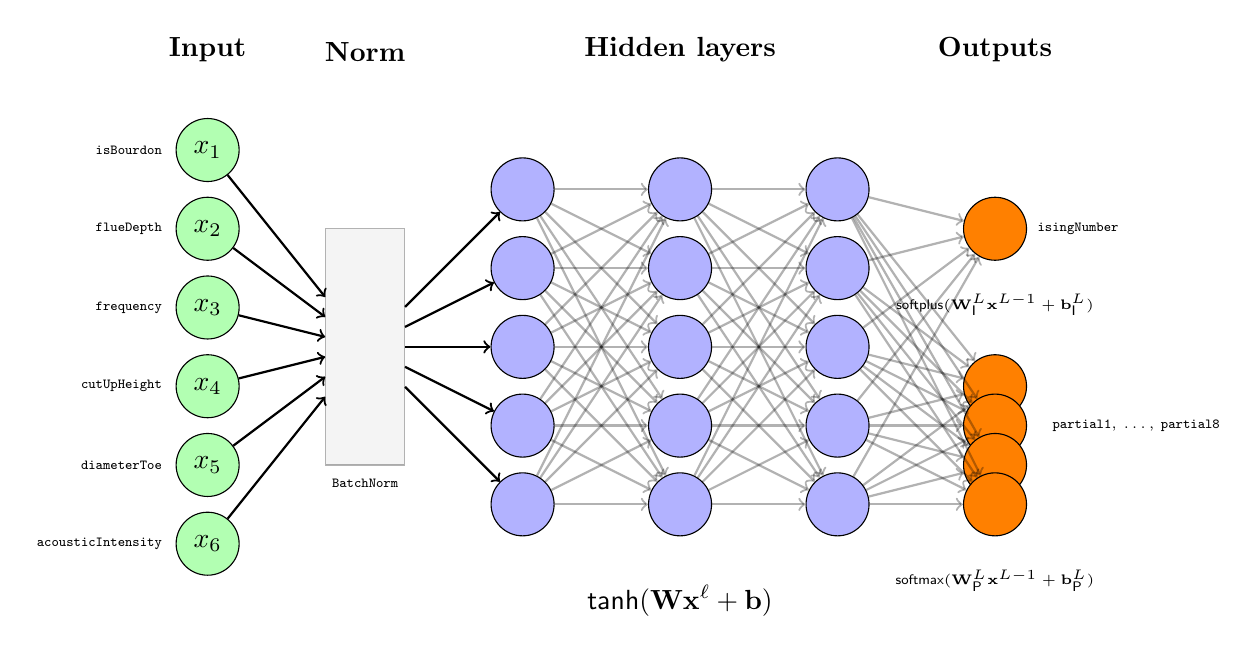
\begin{tikzpicture}[
    node distance=2cm,
    neuron/.style={circle, draw, minimum size=8mm, fill=blue!30},
    input/.style={circle, draw, minimum size=8mm, fill=green!30},
    output/.style={circle, draw, minimum size=8mm, fill=orange},
    layer/.style={rectangle, draw, minimum height=3cm, minimum width=1cm, fill=gray!30, opacity=0.3},
    connection/.style={->, thick}
]

% Input nodes
\node[input] (i1) at (0,3) {$x_1$};
\node[input] (i2) at (0,2) {$x_2$};
\node[input] (i3) at (0,1) {$x_3$};
\node[input] (i4) at (0,0) {$x_4$};
\node[input] (i5) at (0,-1) {$x_5$};
\node[input] (i6) at (0,-2) {$x_6$};

% Input labels
\node[left=0.5mm of i1] {\tiny{\texttt{isBourdon}}};
\node[left=0.5mm of i2] {\tiny{\texttt{flueDepth}}};
\node[left=0.5mm of i3] {\tiny{\texttt{frequency}}};
\node[left=0.5mm of i4] {\tiny{\texttt{cutUpHeight}}};
\node[left=0.5mm of i5] {\tiny{\texttt{diameterToe}}};
\node[left=0.5mm of i6] {\tiny{\texttt{acousticIntensity}}};

% Batch Normalization
\node[layer] (bn) at (2,0.5) {};
\node[below=0.5mm of bn] {\tiny{\texttt{BatchNorm}}};

% Input Layer (6 -> 16)
\node[neuron] (h1_1) at (4,2.5) {};
\node[neuron] (h1_2) at (4,1.5) {};
\node[neuron] (h1_3) at (4,0.5) {};
\node[neuron] (h1_4) at (4,-0.5) {};
\node[neuron] (h1_5) at (4,-1.5) {};
%{\scriptsize tanh};

% Hidden Layer 1 (16 -> 16)
\node[neuron] (h2_1) at (6,2.5) {};
\node[neuron] (h2_2) at (6,1.5) {};
\node[neuron] (h2_3) at (6,0.5) {};
\node[neuron] (h2_4) at (6,-0.5) {};
\node[neuron] (h2_5) at (6,-1.5) {};
\node[below=5mm of h2_5] {\(\mathsf{tanh}(\mathbf{W} \mathbf{x}^\ell + \mathbf{b})\)};

% Hidden Layer 2 (16 -> 16)
\node[neuron] (h3_1) at (8,2.5) {};
\node[neuron] (h3_2) at (8,1.5) {};
\node[neuron] (h3_3) at (8,0.5) {};
\node[neuron] (h3_4) at (8,-0.5) {};
\node[neuron] (h3_5) at (8,-1.5) {};

% Output Branch 1: Ising Number (16 -> 1)
\node[output] (o_ising) at (10,2) {};
\node[right=0.1mm of o_ising] {\tiny{\texttt{isingNumber}}};
\node[below=3mm of o_ising] {\tiny{\(\mathsf{softplus}(\mathbf{W}_{\mathsf{I}}^L \mathbf{x}^{L-1} + \mathbf{b}_{\mathsf{I}}^L)\)}};

% Output Branch 2: Partials (16 -> 8)
\node[output] (o1) at (10,0) {};
\node[output] (o2) at (10,-0.5) {};
\node[output] (o3) at (10,-1) {};
\node[output] (o4) at (10,-1.5) {};
\node[right=2mm of o2] {\tiny{\texttt{partial1}, \dots, \texttt{partial8}}};
\node[below=3mm of o4] {\tiny{\(\mathsf{softmax}(\mathbf{W}_{\mathsf{P}}^L \mathbf{x}^{L-1} + \mathbf{b}_{\mathsf{P}}^L)\)}};

% Connections from inputs to batch norm
\foreach \i in {1,2,3,4,5,6} {
    \draw[connection] (i\i) -- (bn);
}

% Connections from batch norm to first hidden layer
\foreach \i in {1,2,3,4,5} {
    \draw[connection] (bn) -- (h1_\i);
}

% Connections between hidden layers
\foreach \i in {1,2,3,4,5} {
    \foreach \j in {1,2,3,4,5} {
        \draw[connection, opacity=0.3] (h1_\i) -- (h2_\j);
        \draw[connection, opacity=0.3] (h2_\i) -- (h3_\j);
    }
}

% Connections to Ising output
\foreach \i in {1,2,3,4,5} {
    \draw[connection, opacity=0.3] (h3_\i) -- (o_ising);
}

% Connections to Partials outputs
\foreach \i in {1,2,3,4,5} {
    \foreach \j in {1,2,3,4} {
        \draw[connection, opacity=0.3] (h3_\i) -- (o\j);
    }
}

% Layer labels
\node[above=5mm] at (0,3.5) {\textbf{Input}};
\node[above=5mm] at (2,3.5) {\textbf{Norm}};
\node[above=5mm] at (6,3.5) {\textbf{Hidden layers}};
\node[above=5mm] at (10,3.5) {\textbf{Outputs}};

\end{tikzpicture}

\caption{Deep Neural Network Architecture for Ising Number and Partials Prediction}
\label{fig:dnn_architecture}
\end{figure}


\subsection{Hyperparameter tuning}
% TODO: Gabriel has this in /Code/dnnpype

\chapter{Generalized Additive Models and the Ising number}

% TODO: Meghana and Daniel had this

\nocite{*} % This will include all references in the bibliography
\printchicagobibliography

% \chapter*{Notes}
% \addcontentsline{toc}{chapter}{Notes}
% \printchicagonotes

% \appendix

\end{document}
